\documentclass[a4paper,11pt, twoside]{book}

\usepackage[italian]{babel}
\usepackage[utf8x]{inputenc}
\usepackage{graphicx}
\usepackage{float}
\usepackage{url}
\usepackage[writefile]{listings}
\usepackage[Sonny]{fncychap}
\usepackage{fancyhdr}
\usepackage{supertabular}
\usepackage{longtable}
\usepackage[table]{xcolor}
\usepackage{array}
\usepackage{multirow}

\usepackage[italian]{babel}
\usepackage[utf8x]{inputenc}
\usepackage{graphicx}
\usepackage{float}

\usepackage{url}
\usepackage[writefile]{listings}
\usepackage{supertabular}
\usepackage{longtable}
\usepackage{booktabs}
\usepackage[table]{xcolor}


\usepackage{amssymb,amsmath}

\pagestyle{fancy}

%Impostazione capitoletti pagina
%\renewcommand{\chaptermark}[1]%
%{\markboth{\MakeUppercase{Capitolo \thechapter:\ #1}}{}}
%\renewcommand{\sectionmark}[1]%
%{\markright{\MakeUppercase{Sezione \thesection:\ #1}}}

%Impostazione linee di inizio e fine pagina
\renewcommand{\headrulewidth}{0.5pt}
\renewcommand{\footrulewidth}{0.2pt}

\newcommand{\helv}{%
\fontfamily{phv}\fontseries{b}\fontsize{9}{11}\selectfont}

\fancyhf{}
\fancyhead[LE,RO]{\helv \thepage}
\fancyhead[LO]{\helv \rightmark}
\fancyhead[RE]{\helv \leftmark}
\clearpage{\pagestyle{empty}\cleardoublepage}

\lstnewenvironment{xml}{\lstset{basicstyle=\footnotesize, frame=trbl, breaklines=true}}{} 
\begin{document}

  %Inizio Titolo
  \thispagestyle{empty}
    
  \begin{flushright}
    {Università degli Studi di Padova}\linebreak[1]
    \textbf{Corso di Laurea \linebreak Magistrale in Informatica} \linebreak \linebreak \linebreak \linebreak
  \end{flushright}
  
  \begin{center}
    {\texttt{Relazione del progetto per il corso di Sistemi Concorrenti e Distribuiti \linebreak \linebreak \linebreak \linebreak \linebreak}}
  \end{center}
  
  \begin{center}
    \texttt{\huge{\textbf{Simulatore concorrente e distribuito di una competizione di formula 1}}} \linebreak \linebreak \linebreak \linebreak \linebreak \linebreak \linebreak \linebreak \linebreak
  \end{center}
  
  
  \begin{flushleft}
    Studente: Cacco Federico\\Matricola: 624686\\Data: 11 settembre 2013\\Versione: 1.1
  \end{flushleft}

  \newpage
  \pagenumbering{Roman}
  \setcounter{page}{1}
  %Fine titolo
  
  \section*{Diario delle modifiche}
  
  \begin{longtable}{|p{2cm}|p{2cm}|p{2cm}|p{2cm}|}
      \toprule
	\bfseries{MODIFICA} & \bfseries{AUTORE} & \bfseries{DATA} & \bfseries{VERSIONE} \\\hline
      \endfirsthead
      RFOBB-01 & Presenza di un circuito nella competizione \\\hline
      RFOBB-02 & Presenza di piloti nella competizione \\\hline 
      RFOBB-03 & Presenza di un sistema di controllo della competizione \\\hline
      RFOBB-04 & Il circuito deve essere dotato di una pista e della corsia di rifornimento \\\hline
      RFOBB-05 & La pista deve essere soggetta a regole congruenti di accesso \\\hline
      RFOBB-06 & La corsia dei box deve essere soggetta a regole congruenti di accesso \\\hline
      RFOBB-07 & La pista e la corsia box devono essere condivisibili tra i piloti \\\hline
      RFOBB-08 & La pista e la corsia box devono avere tempi di percorrenza verosimili \\\hline
      RFOBB-09 & La pista e la corsia box devono essere soggette a condizioni atmosferiche \\\hline
      RFOBB-10 & I concorrenti devono possedere personali caratteristiche di prestazione  \\\hline
      RFOBB-11 & I concorrenti devono possedere una strategia di gara  \\\hline
      RFOBB-12 & I concorrenti devono possedere una vettura con specifiche caratteristiche prestazionali  \\\hline
      RFOBB-13 & Il sistema di controllo deve riportare lo stato della competizione  \\\hline
      RFOBB-14 & Il sistema di controllo deve riportare le prestazioni e o stato dei piloti  \\\hline
      RFOBB-15 & Il sistema di controllo deve tener traccia delle migliori prestazioni  \\\hline
      RFOBB-16 & Durata e condizione meteo della gara devono essere configurabili  \\\hline
      RFOBB-17 & Presenza di un controllo di terminazione dei concorrenti a fine gara  \\\hline
      \caption{Requisiti funzionali obbligatori}
      \label{tbl:RequisitiFunzionaliObbligatori}
    \end{longtable}
    
  \tableofcontents
  \newpage
  
  \chapter{Introduzione}
    \setcounter{page}{1}
    \pagenumbering{arabic}
    
    \section{Scopo del progetto}
      Il progetto didattico per il corso di Sistemi Concorrenti e Distribuiti consiste nell'analisi, e la
      successiva risoluzione,
      delle problematiche relative alla progettazione di un simulatore concorrente e distribuito 
      di una competizione paragonabile ad una gara Formula 1.
      
      Il sistema da simulare dovrà prevedere:
      \begin{itemize}
	\item Un circuito, possibilmente selezionabile in fase di configurazione, dotato almeno della pista e della corsia di 
	  rifornimento.
	  Entrambe dovranno essere soggette a regole congruenti di accesso, condivisione, 
	  tempo di percorrenza, condizioni atmosferiche, ecc.
	\item Un insieme configurabile di concorrenti, ciascuno con caratteristiche specifiche di prestazione, risorse, 
	  strategia di gara, ecc.
	\item Un sistema di controllo capace di riportare costantemente, consistentemente e separatamente, 
	  lo stato della competizione, le migliori prestazioni (sul giro, per sezione di circuito) e anche la 
	  situazione di ciascun concorrente rispetto a specifici parametri tecnici
	\item Una particolare competizione, con specifica configurabile della durata e controllo di terminazione 
	  dei concorrenti a fine gara.
      \end{itemize}
      
      Si nota subito la natura concorrente del problema, in quanto tra i vari aspetti di cui bisogna tener conto
      nella progettazione vi sono quelli legati ai sorpassi tra piloti impegnati a percorrere lo stesso tratto di pista
      e la gestione dell'accesso alla corsia dei box.
      
      Analogalmente il progetto si presta anche ad alcune valutazioni dal punto di vista della distribuzione, data
      la presenza di almeno 2 blocchi distinti: un primo che si occupa della simulazione della competizione e un secondo
      che si occupa della rappresentazione grafica del suo stato.
      
      Addizionalmente per ottenere una simulazione verosimile
      della competizione 
      vi sono poi tutta una serie di parametri di cui tener conto, 
      come ad esempio le condizioni meteo, le differenti abilità dei piloti e le varie caratteristiche 
      delle vetture.

      
    
    %\section{Struttura del documento}
%TO DO      
    \section{Terminologia}
      Per chiarezza di seguito verranno spiegati alcuni termini usati all'interno della relazione, 
      che altrimenti potrebbero ad una prima lettura sembrare ambigui.
      
      \paragraph{Tracciato}
        Con il termine tracciato si fa riferimento alla carreggiata della pista su cui corrono le vetture di formula 1, 
	comprende anche la corsia dei box.
      
      \paragraph{Circuito}
        Con circuito fa riferimento a un tracciato dove sia stata stabilita una griglia di partenza.
	
      \paragraph{Gara}
        Gara rappresenta l'evento a cui partecipano i piloti di formula uno. Si tratta di un circuito
	su cui sono state impostati un numero totale di giri da eseguire e delle condizioni meteo.
	
      \paragraph{Concorrente}
        Si tratta dell'entità che partecipa alla gara, ogni concorrente è composto da un pilota e da una vettura
	a lui associata.
        
  \chapter{Analisi dei requisiti}
    I requisiti funzionali obbligatori del progetto sono elencati nella tabella \ref{tbl:RequisitiFunzionaliObbligatori}
    
    \begin{longtable}{|p{2cm}|p{8cm}|}
      \toprule
	\bfseries{CODICE} & \bfseries{DESCRIZIONE} \\\hline
      \endfirsthead
      RFOBB-01 & Presenza di un circuito nella competizione \\\hline
      RFOBB-02 & Presenza di piloti nella competizione \\\hline 
      RFOBB-03 & Presenza di un sistema di controllo della competizione \\\hline
      RFOBB-04 & Il circuito deve essere dotato di una pista e della corsia di rifornimento \\\hline
      RFOBB-05 & La pista deve essere soggetta a regole congruenti di accesso \\\hline
      RFOBB-06 & La corsia dei box deve essere soggetta a regole congruenti di accesso \\\hline
      RFOBB-07 & La pista e la corsia box devono essere condivisibili tra i piloti \\\hline
      RFOBB-08 & La pista e la corsia box devono avere tempi di percorrenza verosimili \\\hline
      RFOBB-09 & La pista e la corsia box devono essere soggette a condizioni atmosferiche \\\hline
      RFOBB-10 & I concorrenti devono possedere personali caratteristiche di prestazione  \\\hline
      RFOBB-11 & I concorrenti devono possedere una strategia di gara  \\\hline
      RFOBB-12 & I concorrenti devono possedere una vettura con specifiche caratteristiche prestazionali  \\\hline
      RFOBB-13 & Il sistema di controllo deve riportare lo stato della competizione  \\\hline
      RFOBB-14 & Il sistema di controllo deve riportare le prestazioni e o stato dei piloti  \\\hline
      RFOBB-15 & Il sistema di controllo deve tener traccia delle migliori prestazioni  \\\hline
      RFOBB-16 & Durata e condizione meteo della gara devono essere configurabili  \\\hline
      RFOBB-17 & Presenza di un controllo di terminazione dei concorrenti a fine gara  \\\hline
      \caption{Requisiti funzionali obbligatori}
      \label{tbl:RequisitiFunzionaliObbligatori}
    \end{longtable}

    I requisiti funzionali opzionali del progetto sono invece elencati nella tabella \ref{tbl:RequisitiFunzionaliOpzionali}
    
    \begin{longtable}{|p{2cm}|p{8cm}|}
      \toprule
	\bfseries{CODICE} & \bfseries{DESCRIZIONE} \\\hline
      \endfirsthead
      RFOPZ-01 & Il circuito può essere scelto in fase di configurazione \\\cline{1-2}
      RFOPZ-02 & I piloti devono poter essere configurabili \\\cline{1-2}
      \caption{Requisiti funzionali opzionali}
      \label{tbl:RequisitiFunzionaliOpzionali}
    \end{longtable}
    
  
  \chapter{Progettazione}
    Durante la prima fase di progettazione si è cercato di individuare un modello per rappresentare
    lo scenario dato e le sue principali componenti.
    
    \section{Modello e componenti}
      \subsection{Modello}
	Per prima è stato necessario decidere con che modello rappresentare lo scenario. Dato che lo scopo
	del progetto è quello di concentrarsi sugli aspetti di natura concorrente e distribuita, è stato scelto di utilizzare un
	modello a tempo discreto.
	
	Questo perché nel nostro caso non interessa valutare il sistema facendolo avanzare uno step alla volta, ma
	vogliamo che esso esegua in modo concorrente e in tempo reale, riportando uno stato coerente in determinati istanti.
	
	Ciò porta ad analizzare prima di tutto la granularità del sistema, ovvero ogni quanto deve possibile determinarne un
        stato coerente. Perciò rapportandosi alla realtà della Formula 1, dove lo stato di ogni pilota viene rilevato in determinati 
	settori della pista,
	si è scelto di rappresentare lo stato del sistema non in funzione del tempo ma in funzione della
	posizione dei piloti nella pista. 
	
	Ciò implica che non è più il tempo, ma la distanza percorsa la variabile indipendente tramite la quale si calcolano
	tutti gli altri dati (tra cui appunto il tempo di percorrenza)
	
	I questo modo è possibile determinare dei punti della pista in cui poter recuperare uno stato coerente del sistema,
	analogalmente a quanto succede quando un pilota termina in intermedio in una reale gara di Formula 1.
	Non verrà quindi riportato lo stato del sistema quando un pilota si trova tra 2 intermedi, ma durante questi
	istanti verrà usato un modello di concorrenza per far si che il sistema evolva in modo corretto.
	
	Sulla base di ciò come prima cosa è stata elaborata l'idea di suddividere un tracciato in vari segmenti.
	
      \subsection{Componenti}
	Successivamente si è pensato a come scomporre il sistema, individuandone le varie componenti fondamentali
      
	Per prima cosa sono state individuate 2 partizioni ben distinte, una chiamata F1Engine legata al 
	funzionamento dell'applicazione e una chiamata F1ControlPanel legata alla visualizzazione dello stato della competizione.
	
	La motivazione di questa prima suddivisione risiede nella necessità di poter poi distribuire l'intero sistema,
	creando 2 partizioni che potessero cooperare eseguendo però in modo indipendente l'una dall'altra.
	
	Per ogni partizione del progetto sono state poi individuati i seguenti componenti:
	
	\begin{itemize}
	  \item F1Engine
	  \begin{itemize}
	    \item Gara 
	    \item Concorrenti
	    \item StartUp
	  \end{itemize}
	  \item F1ControlPanel
	  \begin{itemize}
	    \item Monitor
	  \end{itemize}
	\end{itemize}
	
	Questi componenti verranno poi descritti in modo più approfondito per chiarire il loro compito all'interno del
	sistema.
	
    \section{Gara}
      Verrà ora descritto la struttura del componente \textsl{Gara}, con lo scopo di fornire una prima organizzazione gerarchica 
      dei vari componenti e averne quindi una prima visione d'insieme.
      
      La gara come detto rappresenta l'evento alla quale partecipano i vari concorrenti, ed è composta
      da un circuito, una condizione meteo e un numero di giri da percorrere.
      
      Essa non svolge alcun ruolo attivo
      e la sua unica funzione è quella di accogliere i piloti impegnati nella competizione. 
      La gestione della parte concorrente è effettuata mediante dei suoi sotto-componenti. 
      
      Alla base di ciò nella progettazione di Gara si è tenuto conto i questi aspetti:
	
	\begin{itemize}
	  \item Dovrà essere specificata una lunghezza del circuito
	  \item Il circuito deve avere una larghezza variabile durante la sua percorrenza, non in tutti i tratti sarà
		ad esempio possibile eseguire un sorpasso per via dello spazio limitato
	  \item Nel circuito dovranno essere presenti sia tratti curvi che rettilinei, che avranno quindi diverse velocità
		di percorrenza
	  \item Dovranno esserci dei punti per il rilevamento delle prestazioni
	  \item Dovrà essere presente una corsia per i box, con relative regole di accesso
	  \item Le prestazioni possono essere influenzate dalle condizioni meteo
	\end{itemize}
	
      Come detto la componente \textsl{Gara} in se non svolge alcun ruolo attivo, e trattandosi di una semplice
      collezione di dati non necessità di particolari accorgimenti come ad esempio possono richiederne una risorsa protetta
      o un'entità passiva-reattiva. É dunque possibile modellare tale componente come un semplice record di dati 
      che verrà condiviso tra tutti i piloti, contenente i seguenti campi:
      
      \begin{itemize}
	\item Circuito
	\item Numero di giri
	\item Condizioni meteo
      \end{itemize}
      
      \textsl{Numero di giri} è un semplice campo numerico, mentre \textsl{Condizioni meteo} può assumere i 
      valori asciutto o bagnato. Quest'ultimo andrà poi a influenzare il tempo necessario ad un pilota per compiere 
      un giro di pista, in quando con pista bagnata le prestazioni decrescono sensibilmente.
      
      \textsl{Circuito} rappresenta invece il tracciato su cui si svolge la gara, comprendendo la relativa griglia di partenza.
      Come per \textsl{Gara} anche quest'ultimo non ha nessun ruolo attivo e può nuovamente
      essere rappresentato come un semplice record di dati con i seguenti campi:      
      
      \begin{itemize}
	\item Nome del circuito
	\item Numero di segmenti
	\item Lista dei segmenti
	\item Griglia di partenza
	\item Lunghezza del giro
      \end{itemize}
      
      \textsl{Nome del circuito} e \textsl{Lunghezza del giro} sono dei semplici campi che contengono appunto
      il nome del circuito e la lunghezza di ogni giro (corsia dei box esclusa)
      
      Data la necessità di fissare dei punti
      in cui poter recuperare lo stato di un pilota e dato che in un reale circuito 
      di Formula 1 si possono distinguere tratti di pista contigui con caratteristiche simili
      (come ad esempio curve e rettilinei o anche
      tratti che consentono o meno ai vari piloti i sorpassarsi), si è deciso
      di suddividere il tracciato in vari segmenti, che sono appunto tratti di pista contigui con simili caratteristiche.
      Un tracciato è dunque rappresentato come usa successione di questi
      
      Anche \textsl{Griglia di partenza} non è un semplice campo dati, ma si tratta di una entità un po' più complessa
      in quanto rappresenta la griglia di partenza nella quale i piloti si schiereranno nell'attesa del via.
      
      Per chiarezza uno schema della struttura del componente \textsl{Gara} è riportato nella figura \ref{Fig:SchemaGara}
      
      \begin{figure}[h]
	\centering
	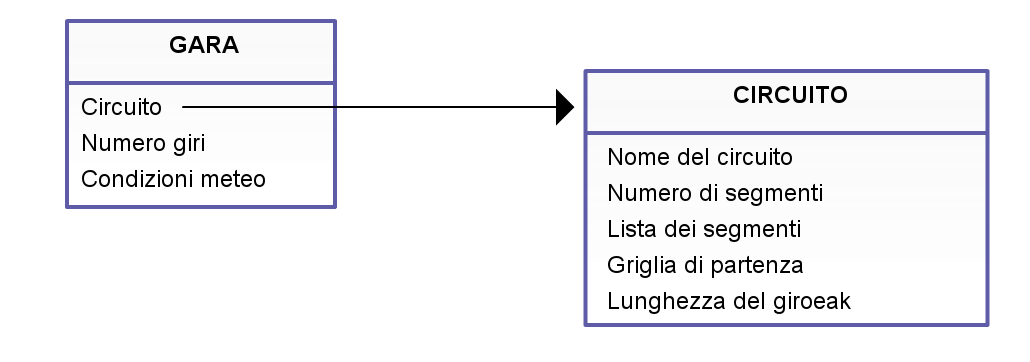
\includegraphics[width=110mm]{./Immagini/SchemaGara.png}
	% SchemaGara.png: 2178x2098 pixel, 72dpi, 76.83x74.01 cm, bb=0 0 2178 2098
	\caption{Schema di Gara}
	\label{Fig:SchemaGara}
      \end{figure}
      
      Ora che è stata data una visione d'insieme dell'intera struttura di \textsl{Gara}, è possibile descriverne con più
      chiarezza i componenti principali.
	
      \subsection{Circuito}
	Come già detto rappresenta il tracciato su cui si svolge la competizione che viene rappresentato come una successione
	di segmenti, e la relativa griglia di partenza.
	
	Sulla base di ciò \textsl{Circuito} contiene quindi le seguenti proprietà:
	
	\begin{itemize}
	  \item Nome del circuito
	  \item Numero di segmenti
	  \item Lista dei segmenti
	  \item Griglia di partenza
	  \item Lunghezza del giro
	\end{itemize}
	  
	\subsection{Lista dei segmenti}
	  Questo parametro contiene la lista dei segmenti di cui è composto il circuito. Nella sua composizione
	  dovranno essere rispettati i seguenti vincoli:
	  
	  \begin{itemize}
	    \item I primi 3 segmenti rappresentano l'ingresso ai box, la corsia box e l'uscita dai box
	    \item Il rettilineo col traguardo deve essere il quarto segmento
	    \item Presenza di almeno 4 intermedi, l'ultimo dei quali coincidente col traguardo
	  \end{itemize}
	  
	  Inoltre si assume che la linea del traguardo sia collocata all'inizio del quarto segmento, che 
	  l'ingresso dei box sia collocato all'inizio del rettilineo del traguardo e che l'uscita box sia collocata
	  alla fine del rettilineo del traguardo.

      \subsection{Segmenti}
	La loro funzione, oltre a quella di descrivere il tracciato su cui si svolge la gara, è quella
	di gestire la parte di concorrenza relativa ai sorpassi tra piloti determinando i loro tempi di attraversamento
	in modo coerente rispetto ala presenza o meno di altri piloti.
	
	Le caratteristiche in base alla quale vengono raggruppati i tratti di pista contigui per dare origine ai segmenti sono:
	\begin{itemize}
	  \item Numero di corsie del tratto di pista
	  \item Tipologia del tratto di pista (accelerazione, frenata, curva, entrata ai box, uscita dai box, corsia dei box)
	\end{itemize}
	
	Il \textsl{numero di corsie} specifica quanti piloti possono attraversare il tratto di pista contemporaneamente uno in 
	fianco all'altro.
	La \textsl{tipologia del tratto di pista} invece rappresenta il modo in cui si deve comportare un pilota quando lo attraversa,
	le varie tipologie sono accelerazione, frenata, curva, entrata ai box, uscita dai box e corsia dei box.
	
	Perciò un segmento è dunque rappresentato da un record contenenti i seguenti campi:
	
	\begin{itemize}
	  \item Codice segmento
	  \item Tipologia
	  \item Lunghezza
	  \item Velocità massima
	  \item Numero di corsie
	  \item Presenza fotocellula
	  \item Risorsa protetta
	\end{itemize}
	
	\subsubsection{Codice segmento}
	  Serve per poter distinguere i vari segmenti tramite un codice univoco crescente che ne determina il loro ordinamento
	  nella composizione del circuito. 

	  Per semplicità di implementazione si è scelta la seguente numerazione dei segmenti
	  \begin{itemize}
	    \item 1: il segmento di entrata ai box
	    \item 2: il segmento della corsia dei box
	    \item 3: il segmento di uscita dai box
	    \item 4: il segmento del rettilineo principale (quello in cui è presente il traguardo)
	    \item i>4: gli altri segmenti che vengono dopo il traguardo
	  \end{itemize}
	  
	\subsubsection{Tipologia}
	  Un segmento deve essere in grado di rappresentare il più fedelmente possibile il tratto di pista
	  a lui corrispondente. Compatibilmente con i requisiti del progetto sono state individuate 3 classi
	  di tipologia di segmento:
	  
	  \begin{itemize}
	    \item Segmenti di accelerazione
	    \item Segmenti a velocità costante
	    \item Segmenti di decelerazione
	  \end{itemize}
	  
	  I segmenti di accelerazione modellano tratti in cui i piloti accelerano, ovvero rettilinei e uscita dai box. I segmenti di
	  decelerazione modellano invece ingressi in curva, staccate e corsia di entrata ai box. Infine
	  i segmenti a velocità costanti modellano curve e corsia dei box.
	  
	\subsubsection{Lunghezza}
	  Descrive semplicemente la lunghezza in metri del segmento
	
	\subsubsection{Velocità massima}
	  Il significato di questo dato varia in base alla tipologia del segmento. Nel caso
	  in cui esso sia associato ad un segmento di accelerazione indica la massima velocità che la vettura può raggiungere,
	  questo è utile ad esempio per modellare rettilinei non completamente dritti.
	  Nei segmenti di decelerazione la velocità massima indica invece la velocità che dovrà avere la vettura al termine del
	  segmento, per poter poi effettuare una curva o entrare in un segmento a velocità controllata come ad esempio la
	  corsia dei box.
	  Infine nei tratti a velocità costante il valore rappresenta la velocità massima con cui il segmento potrà essere
	  attraversato, e avrà lo stesso valore del precedente tratto di decelerazione.
	  
	  Un tratto a velocità costante deve essere sempre preceduto da un tratto di decelerazione o di accelerazione
	  che abbia la sua stessa velocità massima. Concettualmente è molto simile ad un tratto di accelerazione
	  con velocità massima limitata, però tale distinzione risulterà poi comoda a livello implementativo
	  per risparmiar inutili calcoli di accelerazione.
	  
	  Tutti i valori della velocità massima sono solo indicativi e servono per dare una descrizione del segmento,
	  i reali valori di attraversamento verranno calcolati anche in base alle caratteristiche e allo stato di 
	  vettura e pilota, come sarà spiegato nella sezione \ref{AttraversamentoSegmenti}
	    
	\subsubsection{Numero di corsie}
	  Rappresenta il numero di corsie presenti nel segmento, influenzando la possibilità
	  di poter effettuare sorpassi da parte dei piloti. Il loro numero determina infatti quanti piloti possono trovarsi
	  contemporaneamente nello stesso tratto di segmento
	  
	  In un segmento con una sola corsia sarà dunque impossibile effettuare sorpassi, mentre saranno più agevoli
	  al loro aumentare.
	  
	  Le corsie d'ingresso e uscita dai box, la corsia dei box e le curve hanno sempre il numero di corsie pari
	  a 1
	  
	\subsubsection{Presenza fotocellula}
	  Un circuito di Formula uno è solitamente diviso in 4 intermedi, alla fine dei quali
	  è presente un dispositivo per rilevare i tempi dei vari piloti. Questo parametro
	  indica se alla fine del segmento deve essere rilevato tale tempo, e in caso affermativo
	  specifica anche il numero dell'intermedio alla quale tale tempo si riferisce.
	

	\subsubsection{Risorsa protetta}
	  Ogni segmento contiene al suo interno una risorsa protetta, che ha essenzialmente due compiti. Il primo
	  è quello di rendere possibile un accesso ai segmenti congruente ai vari vincoli imposti, 
	  il secondo è quello di permettere un ordinamento dei piloti in base alla loro posizione.
	  
	  Una spiegazione dettagliata del loro funzionamento sarà data nella sezione \ref{Accesso ai segmenti}
	  
      \subsection{Griglia di partenza}
	La griglia di partenza è il luogo dove i piloti prendono posto attendendo l'inizio della gara, ed è anch'essa modellata
	mediante una risorsa protetta.
	Il suo funzionamento verrà spiegato nella sezione \ref{Schieramento nella griglia di partenza}
	  
    \section{Piloti}
      I piloti sono le entità che dovranno gareggiare nella competizione attraversando il circuito.
      Lo scopo di ognuno d'essi è quello di percorrere tutti i giri previsti nella gara nel minor tempo possibile,
      il tutto in modo coerente con le caratteristiche del circuito.
      
      Dato che nella realtà ogni pilota ha le proprie abilità (come ad esempio la prontezza di riflessi
      o la capacità di valutare i punti esatti in cui effettuare le staccate),
      anche in questo caso ad ogni pilota dovranno essere associate delle caratteristiche, chiamate skill, che possano
      modellarne il comportamento in pista. Le skill che ogni pilota possiede sono:
      
      \begin{itemize}
	\item Numero del pilota
	\item Nome del pilota
	\item Skill di accelerazione
	\item Skill di decelerazione
      \end{itemize}
      
      La skill di accelerazione e la skill di decelerazione indicano rispettivamente la capacità del pilota di 
      iniziare l'accelerazione 
      il più presto possibile e la capacità del pilota di frenare 
      il più tardi possibile prima di un inserimento in curva. Bassi valori in queste skill implicheranno che il pilota 
      inizia ad accelerare troppo tardi e a frenare troppo presto 
      rispetto all'istante ottimale, peggiorando così le sue prestazioni nel giro di pista.
      
      Ad ogni pilota viene poi associata una vettura, anch'essa caratterizzata da delle skill che ne influenzeranno
      le prestazioni in pista. Esse sono:
      
      \begin{itemize}
	\item Costruttore
	\item Coefficiente di accelerazione
	\item Coefficiente di decelerazione
	\item Velocità massima
	\item Tenuta di strada
	\item Consumo degli pneumatici
      \end{itemize}
      
      I coefficienti di accelerazione e di decelerazione indicano le prestazioni di accelerazione e frenata della vettura, 
      vetture con alti coefficienti avranno quindi migliori capacità di accelerazione e decelerazione
      che comporteranno prestazioni migliori.
      
      La tenuta di strada viene invece usata per calcolare i tempi di percorrenza nelle curve e quanto peggiorano 
      le prestazioni in caso di pista bagnata.
      
      Il consumo degli pneumatici invece stabilisce in quanti giri essi degradano e hanno quindi bisogno di essere sostituiti
      ai box. Vetture con un basso degrado degli pneumatici potranno compiere più giri senza doversi fermare ai box.
      
      Ogni pilota inoltre possiede un propria strategia, che rappresenta l'elenco dei giri in cui fermarsi per effettuare il
      cambio gomme. E' importante bilanciare il vantaggio di avere sempre pneumatici in buone condizioni con lo svantaggio
      di doversi fermare per sostituirli.
      
      Infine piloti che utilizzano vetture con un basso consumo di carburante potranno completare la gara
      immagazzinando alla partenza un minor quantitativo d'esso, rendendo così la vettura più leggera e performante.
      
      \subsection{Simulazione accelerazione}
	Dato che simulare la reale curva di accelerazione di una vettura di formula è una operazione complessa,
	è stato deciso di semplificarne la sua rappresentazione.
	L'aspetto chiave da tenere in considerazione è il fatto che la fora di accelerazione varia in funzione della velocità,
	più precisamente più bassa è la velocità e maggiore è l'accelerazione che si riesce ad imprimere alla vettura
	
	In più, dato che tutto il sistema di riferimento è in base allo spazio percorso e non al tempo, la velocità
	viene calcolata in base alla distanza percorsa e non in base al tempo.
	
	La funzione scelta per rappresentare la velocità $v$ in funzione della distanza $x$ percorsa è 
	dunque la seguente:
	
	$$v(x)=80*log[(\frac{x}{100})+1]$$
	
	La funzione inversa per calcolare lo spazio percorso $x$ in funzione della velocità raggiunta $v$ è invece:
	
	$$x(v)=100*[10^{(v/80)}-1]$$
	
	Il tempo necessario all'attraversamento viene poi calcolato ipotizzando di attraversare il segmento ad una velocità
	costante pari alla media tra la velocità di ingresso e quella d'uscita.
		
	Nella figura \ref{fgr:GraficoVelocita} viene rappresentato il grafico della funzione usata per simulare il valore
	della velocità raggiunta in funzione della distanza percorsa.
	
	\begin{figure}[h]
	  \centering
	  \fbox{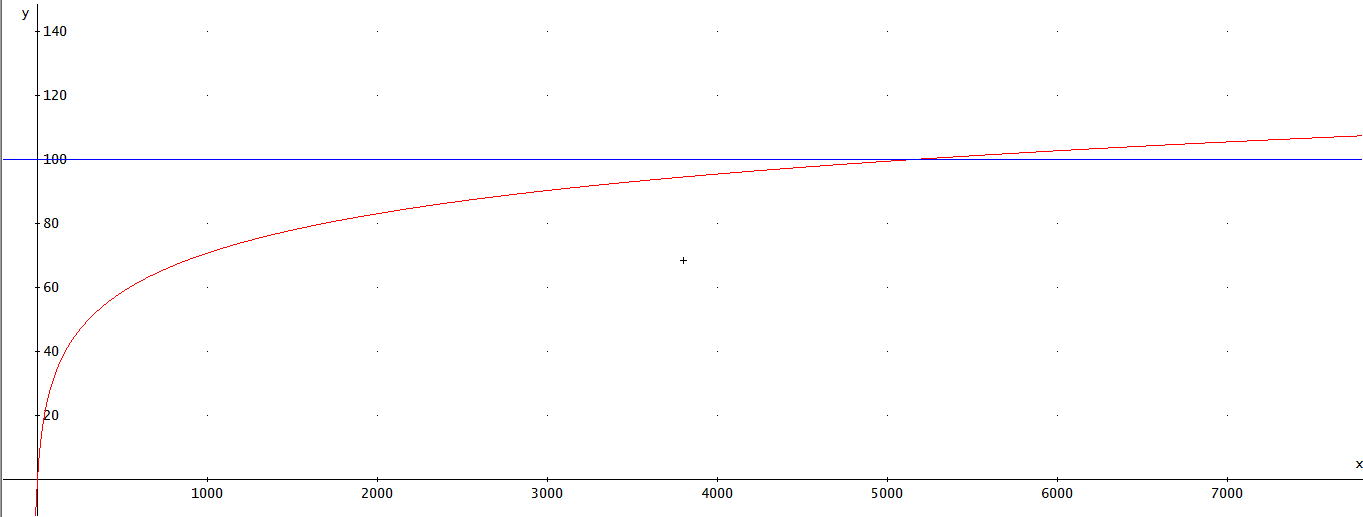
\includegraphics[width=120mm]{./Immagini/GraficoVelocita.png}}
	  % GraficoVelocità.png: 1363x517 pixel, 99dpi, 34.97x13.26 cm, bb=0 0 991 376
	  \caption{Andamento della velocità in base alla distanza percorsa di una vettura con velocità iniziale
		    pari a 0m/s}
	  \label{fgr:GraficoVelocita}
	\end{figure}
	
	Tale grafico presuppone che la vettura parta da una velocità iniziale di 0m/s, ma questo si verifica solo 
	alla partenza.
	Per calcolare la variazione di velocità della vettura in funzione della distanza percorsa, nel caso in cui la vettura
	abbia una velocità iniziale $v_0$ diversa da 0 è sufficiente traslare il grafico fino a intersecare tale valore $v_0$
	con l'asse delle ordinate, come nell'esempio in figura \ref{fgr:GraficoVelocitaTraslato}
	
	\begin{figure}[h]
	  \centering
	  \fbox{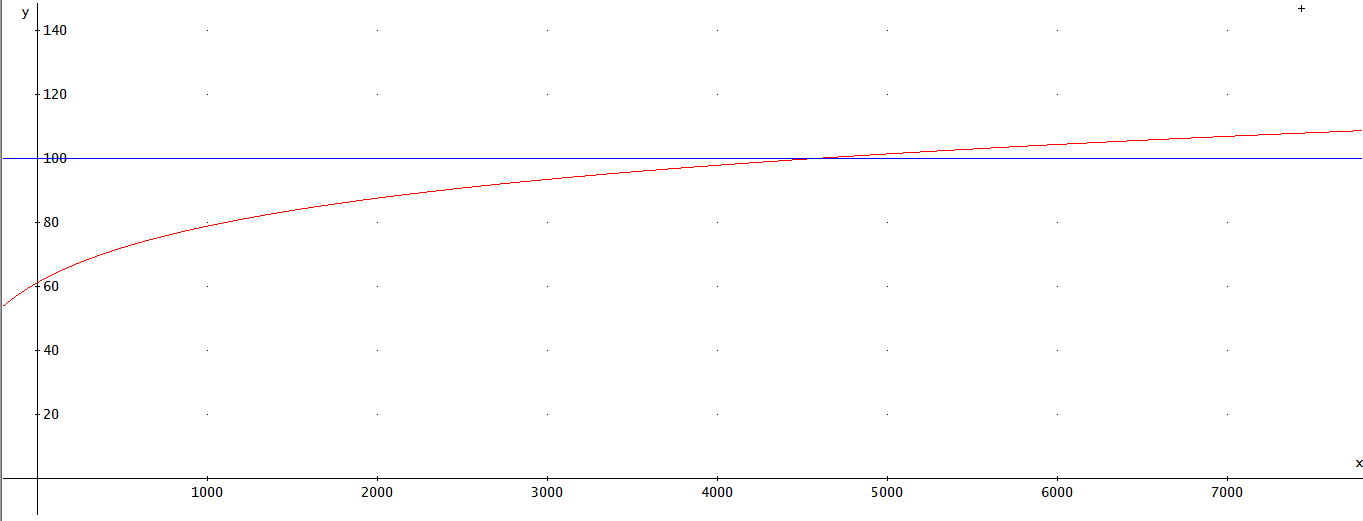
\includegraphics[width=120mm]{./Immagini/GraficoVelocitaTraslato.png}}
	  % GraficoVelocità.png: 1363x517 pixel, 99dpi, 34.97x13.26 cm, bb=0 0 991 376
	  \caption{Andamento della velocità in funzione della distanza, assumendo che la vettura abbia una
		    velocità iniziale $v_0$ di 60m/s}
	  \label{fgr:GraficoVelocitaTraslato}

	\end{figure}

      \subsection{Simulazione decelerazione}
	La simulazione della decelerazione risulta molto più semplice rispetto a quella dell'accelerazione in quanto
	si può approssimare il fatto che durante la frenata la forza impressa dal freno sia costante.
	
        La simulazione di una decelerazione viene effettuata calcolando per prima cosa lo spazio necessario alla frenata,
	in modo da determinare per quanto spazio il pilota continuerà ad accelerare e per quando spazio 
	eseguirà la frenata. Ad ogni vettura è associato quindi
	un coefficiente $EffDec$, che misura la forza sua forza di decelerazione
	
	La formula con la quale essa viene calcolato lo spazio di frenata $x$ necessario per effettuare una variazione 
	di velocità $\Delta V$ alla velocità iniziale $v_i$ è la seguente:
	
	$$x(\Delta V)=\frac{1}{2}*EffDec*\frac{\Delta V^2}{EffDec^2}+v_i*\frac{\Delta v}{EffDec}$$
	
	Il tempo necessario per effettuare la frenata sarà invece
	
	$$t(\Delta v) = \frac{\Delta v}{DecEff}$$

		
      \subsection{Simulazione tratto a velocità costante}
        
        Il questo caso per calcolare il tempo di attraversamento di usano le leggi del moto rettilineo uniforme,
	dove $v$ è la velocità di attraversamento e $l$ la lunghezza del segmento
	
	$$t(v)=l/v$$
	
      \subsection{Azioni del pilota}
        Nel loro ciclo di vita i piloti compiono le seguenti azioni:
	
	\begin{itemize}
	  \item Schieramento nella griglia di partenza
	  \item Partenza
	  \item Attraversamento dei segmenti
	  \item Eventuali soste ai box
	  \item Terminazione della gara
	\end{itemize}

	\subsubsection{Schieramento nella griglia di partenza}
	  Questa è la prima fase della gara, semplicemente una volta che il pilota è stato creato
	  viene posizionato nella griglia di partenza nell'attesa di iniziare la gara.
	  
	\subsubsection{Partenza}
	
	  Una volta tutti i piloti sono schierati nella griglia di partenza il sistema resta in attesa di un input
	  da parte dell'utente per poter dare inizio alla gara.
	  
	  Appena ricevuto il segnale i piloti partono e iniziano l'attraversamento dei segmenti.
	  
	\subsubsection{Attraversamento dei segmenti}
	\label{AttraversamentoSegmenti}
	  In questa fase i piloti attraversano i vari segmenti del tracciato nel tentativo di completare tutti i giri
	  nel minor tempo possibile.
	  
	  L'Attraversamento di un segmento si svolge in modo analogo sia che il tratto di pista sia
	  di accelerazione, di frenata o a velocità costante (curva). Cambia solo il modo con cui esso viene 
	  determinato il tempo di attraversamento.
	  
	  Nel caso in cui il pilota sia impegnato in un tratto di a velocità costante
	  il tempo di attraversamento viene calcolato nel seguente modo:
	  
	  \begin{enumerate}
	    \item In base alla velocità del pilota e alla lunghezza del segmento viene calcolato il tempo di attraversamento previsto
	    \item Si calcolano poi delle penalità che verranno aggiunte a tale tempo, che sono:
		  \begin{itemize}
		    \item Condizioni meteo e tenuta di strada (max 10\% del tempo calcolato)
		    \item Stato degli pneumatici (max 4\% del tempo calcolato)
		    \item Peso della benzina nella vettura (0,05\% in più del tempo per ogni litro nel serbatoio)
		  \end{itemize}
		  Tali penalità vengono poi sommate al tempo di attraversamento
	    \item A questo punto il pilota chiede l'accesso alla risorsa protetta del segmento
		  comunicando il tempo atteso per l'attraversamento. La risorsa risponde comunicando il tempo
		  effettivo di attraversamento sulla base della presenza o meno di altri piloti
	  \end{enumerate}
	  
	  Nel caso invece in cui il pilota sia impegnato in un tratto di accelerazione i passi
	  per calcolare il tempo necessario al suo attraversamento sono:
	  
	  \begin{enumerate}
	    \item In base alle caratteristiche del pilota viene calcolato lo spazio di ritardo con cui il
		  pilota inizierà l'accelerazione. Tale spazio potrà essere al massimo il 10$\%$ della lunghezza del segmento
	    \item Viene quindi calcolato lo spazio effettivo di accelerazione, che sarà quindi tanto maggiore quanto
		  il pilota sarà abile nell'accelerare il prima possibile
	    \item In base dello spazio di accelerazione effettivo viene calcolata la velocità massima che il pilota avrà alla fine del 
		  tratto di accelerazione,
		  tale velocità sarà ridotta al massimo del 10$\%$ sulla base delle prestazioni in accelerazione della vettura,
		  e non sarà comunque superiore alla velocità massima della vettura
	    \item Sulla base della velocità di entrata del segmento e di quella di uscita si calcola il tempo di attraversamento
	    \item Si calcolano poi delle penalità che verranno aggiunte a tale tempo, che sono:
		  \begin{itemize}
		    \item Condizioni meteo e tenuta di strada (max 10\% del tempo calcolato)
		    \item Stato degli pneumatici (max 4\% del tempo calcolato)
		    \item Peso della benzina nella vettura (0,05\% in più del tempo per ogni litro nel serbatoio)
		  \end{itemize}
		  Tali penalità vengono poi sommate al tempo di attraversamento
	    \item A questo punto il pilota chiede l'accesso alla risorsa protetta del segmento
		  comunicando il tempo atteso per l'attraversamento. La risorsa risponde comunicando il tempo
		  effettivo di attraversamento sulla base della presenza o meno di altri piloti
	  \end{enumerate}
	  
	  Infine nel caso in cui il pilota sia impegnato in un tratto di decelerazione il procedimento è il seguente:
	  
	  \begin{enumerate}
	    \item Viene calcolato lo spazio di frenata in base alla skill di frenata dell'auto
	    \item In base alle caratteristiche del pilota viene calcolato lo spazio di anticipo con cui il
		  pilota inizierà la decelerazione. Tale spazio potrà essere al massimo il 10\% della lunghezza del segmento
		  Maggiore è questo spazio maggiore sarà l'anticipo della frenata, fatto che causerà una diminuzione delle prestazioni.
	    \item Viene quindi calcolato lo spazio effettivo di frenata, che sarà quindi tanto minore quanto
		  il pilota sarà abile nel frenare il più tardi possibile
	    \item In base allo spazio di frenata effettivo viene calcolato il tempo di attraversamento atteso, tale valore
	          verrà poi modificato in base alle skill del pilota e alle caratteristiche della vettura
	    \item Si calcolano poi delle penalità che verranno aggiunte a tale tempo, che sono:
		  \begin{itemize}
		    \item Condizioni meteo e tenuta di strada (max 10\% del tempo calcolato)
		    \item Stato degli pneumatici (max 4\% del tempo calcolato)
		    \item Peso della benzina nella vettura (0,05\% in più del tempo per ogni litro nel serbatoio)
		  \end{itemize}
		  Tali penalità vengono poi sommate al tempo di attraversamento
	    \item A questo punto il pilota chiede l'accesso alla risorsa protetta del segmento
		  comunicando il tempo atteso per l'attraversamento. La risorsa risponde comunicando il tempo
		  effettivo di attraversamento sulla base della presenza o meno di altri piloti
	  \end{enumerate}
	  
	  

	\subsubsection{Soste ai box}
    
	  I piloti avranno poi una loro personale strategia di gara, questo consentirà loro di effettuare
	  i sorpassi non solo durante la percorrenza del giro, ma anche mediante le soste ai box.
	  La strategia di gara specifica la benzina iniziale che la vettura avrà nel serbatoio a inizio gara,
	  e i giri in cui ci si fermerà per il cambio degli pneumatici.
	  
	  Entrambi i fattori sono importanti. Bisognerà sia caricare il minimo quantitativo di benzina necessario per
	  portare a termine la gara (avendo così la vettura il più leggera possibile) e sia
	  schedulare al meglio le soste ai box per il cambio pneumatici, tenendo presente che con pneumatici usurati le prestazioni
	  decrescono in maniera significativa ma allo steso la sosta ai box per la loro sostituzione è un'operazione
	  che richiede una certa quantità di tempo.
	  
	  Dato che nelle competizioni reali le soste ai box sono diventate estremamente veloci (specialmente dopo il divieto di poter
	  effettuare rifornimenti di carburante),
	  nel sistema progettato una sosta ai box viene simulata mediante l'attraversamento della corsia box a velocità ridotta.
	  
	\subsubsection{Fine della gara}
	  Molte volte nelle competizioni di Formula 1 un pilota termina la propria gara non perché
	  abbia completato tutti i giri previsti, ma a causa di altri eventi come ad esempio incidenti,
	  gusti o altro.
	  
	  Volendo riportare questa caratteristica anche nel progetto, sono stati fissati 3 motivi per i quali un 
	  pilota può terminare la propria gara, e sono:
	  
	  \begin{itemize}
	   \item Completamento di tutti i giri previsti
	   \item Fine della benzina
	   \item Guasto nella vettura
	  \end{itemize}
	  
	  Ogni volta che si conclude il giro viene fatto un controllo per determinare se il pilota
	  ha abbastanza benzina per completare un altro giro. In caso affermativo esso procede normalmente
	  effettuando il giro successivo, in caso contrario esso si ritira dalla competizione terminando così la sua gara
	  
	  In base all'affidabilità della vettura poi un pilota ha una certa probabilità che durante la percorrenza del giro
	  la sua vettura possa rompersi causandone il suo ritiro
	
      \subsection{Invio dello stato del pilota}
	Il pilota inoltre in determinati momenti invia delle informazioni sul suo stato al monitor, 
	che poi le elabora per la loro visualizzazione a video.
	
	Le informazioni trasmesse da un pilota sono le seguenti:
	
	\begin{itemize}
	  \item Schieramento del pilota nella griglia di partenza
	  \item Comunicazione del tempo fatto registrare in un determinato intermedio
	  \item Ingresso ai box
	  \item Uscita dai box
	  \item Comunicazione della benzina rimasta e dello stato degli pneumatici
	  \item Comunicazione di gara terminata da parte del pilota
	\end{itemize}
	
	Nella sezione \ref{Comunicazione} si spiegherà come queste informazioni vengono effettivamente inviate al monitor
	
    \section{Monitor}
      Il monitor è una semplice interfaccia grafica che raccoglie le informazioni sullo stato dei piloti ordinati secondo
      la loro posizione.
      
      Essa è modellata come un'entità reattiva, in quando il suo unico compito è quello di ricevere i messaggi
      sullo stato della competizione e riportarli a video.
      
      Le informazioni vengono visualizzate in una tabella dove ad ogni riga è associato un pilota, per ognuno di essi
      viene visualizzato:
      \begin{itemize}
	\item Nome Pilota
	\item Numero
	\item Costruttore
	\item Tempo primo intermedio
	\item Tempo secondo intermedio
	\item Tempo terzo intermedio
	\item Tempo al traguardo
	\item Distacco dal primo
	\item Numero giri fatti
	\item Stato del pilota (in gara, ai box o ritirato)
	\item Numero soste ai box fatte
	\item Carburante presente nel serbatoio
	\item Usura delle gomme
	\item Strategia del pilota (elenco dei giri in cui si fermerà)
	\item Tempo di gara (Visualizzato solo quando il pilota termina la competizione)
      \end{itemize}
      
      Vengono inoltre visualizzate informazioni come nome del circuito, tempo meteorologico, numero di giri previsti,
      stato della gara e miglior giro effettuato

      Il modo con cui tale informazioni vengono raccolte è spiegato nella sezione \ref{Comunicazione}
    
    \section{StartUp}
      Il componente StartUp si occupa della creazione di Gara e piloti e dell'avvio della competizione.
      Esso è l'unico metodo invocato dal main di F1Engine e ha il seguente ciclo di vita:
      
      \begin{enumerate}
	\item Creazione della gara
	\item Creazione dei piloti
	\item Attesa schieramento dei piloti sulla griglia di partenza
	\item Attesa della conferma da parte dell'utente per la partenza
	\item Attesa della fine della gara
	\item Terminazione a fine gara
      \end{enumerate}
      
  \chapter{Distribuzione}
    \section{Partizionamento}
      Il progetto svolto si presta ad alcune considerazioni sull'aspetto della distribuzione. 
      Si può infatti notare che esso è strutturato in 2 parti ben distinte, una contenente la logica della
      competizione (piloti e gara), e una contenente il monitor per la visualizzazione dello
      stato della competizioni.
      
      Inoltre entrambi i blocchi sono indipendenti uno dall'altro. I piloti possono infatti
      gareggiare anche senza la presenza del monitor, mentre quest'ultimo può eseguire anche senza che nessun pilota
      stia gareggiando (ovviamente non mostrerà nessun dato).
      
      Tale suddivisione è inoltre giustificata dal fatto che le parti che richiedono un certo carico computazionale 
      (seppur modesto) sono quelle relative ai piloti e al monitor, mentre
      Gara, trattandosi di una collezione di record di memoria e di risorse protette, ha solamente un ruolo passivo
      e richiede perciò una capacità di calcolo molto inferiore
      
      Queste considerazioni hanno portato quindi a scomporre il progetto in 2 nodi così composti:
      
      \begin{itemize}
	\item Nodo 1:
	\begin{itemize}
	  \item Piloti
	  \item Gara
	\end{itemize}
	\item Nodo 2:
	\begin{itemize}
	  \item Monitor
	\end{itemize}
      \end{itemize}
          
    \section{Comunicazione}
    \label{Comunicazione}
      Una parte fondamentale della distribuzione riguarda la scelta del meccanismo di scambio informazioni tra i 2 nodi.
      
      Nel nostro caso le informazioni scambiate hanno una sola direzione, in quanto il monitor ha il solo compito di
      ricevere le informazioni dal nodo F1Engine e mostrarle a video.
      
      Dato che molte informazioni vengono inviate dal pilota, non è desiderabile che esso
      attenda la risposta di avvenuta ricezione del messaggio da parte del monitor,
      in quando questo trasformerebbe l'operazione di invio messaggio in una operazione bloccante, influenzando così
      in modo indesiderato il suo comportamento.
      
      Un altra considerazione riguarda il fatto che un'informazione non ricevuta o ricevuta in ritardo 
      non causerebbe un'inconsistenza dello stato della competizione a livello logico,
      ma solo una inconsistenza dei dati mostrati a video. Tale fenomeno si risolverebbe poi mano a mano che la gara avanza
      e che i nuovi dati aggiornati vengono ricevuti.
      
      Tali considerazioni suggeriscono quindi la possibilità di usare una comunicazione asincrona nello scambio dei messaggi
      tra i 2 nodi basata su chiamate a procedure remote, con semantica oneway best-efford
            
      Uno schema della distribuzione è riportato nella figura \ref{Fig:SchemaDistribuzione}
      
      \begin{figure}[h]
	\centering
	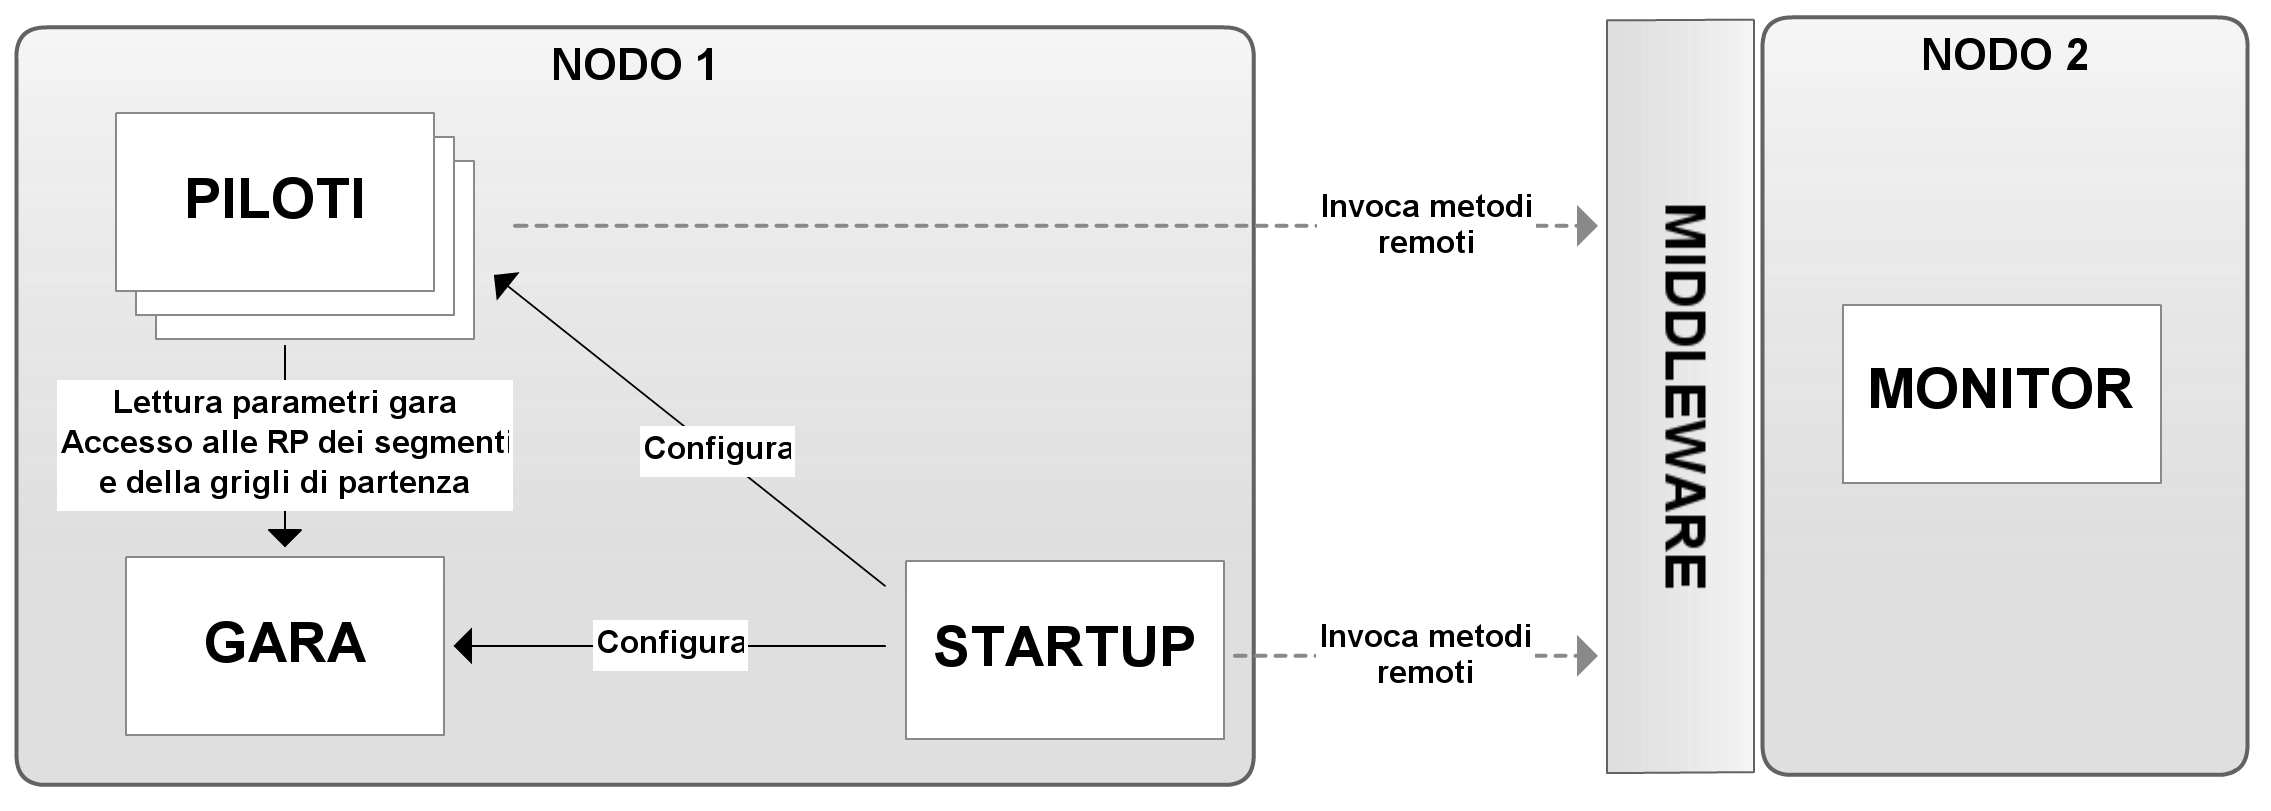
\includegraphics[width=120mm]{./Immagini/SchemaDistribuzione.png}
	% SchemaDistribuzione.png: 2178x792 pixel, 72dpi, 76.83x27.94 cm, bb=0 0 2178 792
	\caption{Schema di distribuzione del progetto}
	\label{Fig:SchemaDistribuzione}
      \end{figure}
  
    
  \chapter{Concorrenza}
  \label{Concorenza}
    Gli aspetti del progetto in cui entrano in gioco problemi di natura concorrenziale sono i seguenti:
    
    \begin{itemize}
      \item Schieramento nella griglia di partenza
      \item Attraversamento dei segmenti da parte dei piloti
    \end{itemize}
    
    \section{Schieramento nella griglia di partenza}
    \label{Schieramento nella griglia di partenza}
      La griglia di partenza è stata modellata come una risorsa protetta, in modo da potervi accodare i piloti
      nell'attesa della partenza, questo è stato necessario in quanto la gara può partire solo una volta che tutti i piloti sono stati schierati,
      
      La risorsa protetta contiene 3 canali d'accesso:
      \begin{itemize}
	\item Uno pubblico sempre aperto chiamato Place\_On\_Grid
	\item Uno privato controllato da una guardia chiamato  Wait\_To\_Start, inizialmente chiusa
	\item Uno pubblico controllato da guardia chiamato Wait\_To\_Pilots, inizialmente chiusa
      \end{itemize}
      
      Il protocollo d'accesso alla griglia di partenza è il seguente, e comprende 2 serie di eventi
      concorrenti:
      
      Thread di gestione della gara
      \begin{itemize}
	\item Una volta che ha creato tutti i piloti chiede accesso al canale Wait\_To\_Pilots,
	      inizialmente con guardia chiusa
	\item Una volta che tutti i piloti sono schierati la guardia di Wait\_To\_Pilots viene aperta e il controllore
	      si pone in attesa del segnale di inizio gara da parte dell'utente
	\item Una volta ricevuto tale segnale viene aperta la guardia Wait\_To\_Start
      \end{itemize}
      
      Thread dei piloti:
      \begin{itemize}
	\item Un pilota viene creato e chiede di schierarsi nella griglia di partenza tramite il canale Place\_On\_Grid,
              il numero di piloti in griglia viene aumentato di uno
	\item Il pilota viene poi riaccordato nel canale Wait\_To\_Start, inizialmente chiuso
	\item Quando il numero dei piloti schierati è uguale al numero di piloti che devono prendere parte alla gara
	      la guardia di Wait\_To\_Pilots viene aperta
	\item I piloti attendono ora l'apertura della guardia Wait\_To\_Start da parte del controllore
      \end{itemize}

	    
    \section{Acceso ai segmenti}
    \label{Accesso ai segmenti}
      L'accesso ai segmenti è la parte cruciale di tutto il sistema in quanto tramite essi viene gestita
      tutta la dinamica della gara, ovvero tempi di percorrenza del circuito, sorpassi e accesso ai box.
      Fornisce inoltre il meccanismo di ordinamento dei piloti durante la competizione
      
      Come detto un segmento è composto da una o più corsie gestite mediante una risorsa protetta per garantire
      l'accesso in mutua esclusione, esse consentono ai piloti di entrare nello stesso segmento 
      contemporaneamente e di effettuare sorpassi.
      Se un segmento è composto da una sola corsia i piloti dovranno necessariamente accodarsi in un'unica fila e attraversare
      il segmento senza alcuna possibilità di effettuare sorpassi.
      
      L'accesso viene modellato mediante una risorsa protetta associata a ciascun segmento, che contiene
      la rappresentazione delle sue corsie e il loro stato. Lo stato della risorsa protetta associata al segmento
      consiste nella memorizzazione dell'istante in cui l'ultimo pilota che vi ha chiesto l'accesso uscirà dalla corsia.
      
      Inoltre ad ogni segmento è assegnato un contatore, che eroga dei ticket decrescenti ai piloti ogni volta ognuno di
      essi esce dal segmento. In questo modo è possibile ordinare i piloti con relativa semplicità senza
      dover tenere in considerazioni alcun aspetto legato al calcolo dei tempi. 
      
      I piloti vengono infatti ordinati, nel momento in cui escono dai segmenti aventi la fotocellula per il rilevamento dei tempi,
      in base al giro in cui sono, al segmento in cui si trovano e al ticket in loro possesso.
      Il caso più difficile è quando si confrontano 2 piloti nello stesso giro usciti dallo stesso segmento,
      rendendo così necessario analizzare il momento temporale in cui sono usciti. Con l'utilizzo dei ticket sarà invece
      sufficiente vedere chi dei 2 ha il ticket più alto, in quanto vorrà dire che sarà quello uscito prima dal segmento.
      
      La modalità d'accesso ai segmenti non varia in base alla sua tipologia, restando la medesima per ognuno d'essi.
      
      Per semplicità il protocollo d'accesso ad un segmento da parte di un pilota è il seguente:
      
      \begin{itemize}
	\item Reperimento delle informazioni del segmento
	\item Calcolo del tempo di attraversamento ideale $T_i$ in base al suo stato e alle caratteristiche del segmento
	\item Accesso in mutua esclusione alla risorsa protetta del segmento
	\item Chiamata alla procedura d'ingresso al segmento della risorsa protetta del segmento, che risponderà comunicando 
	      il reale tempo di attraversamento $T_r$ calcolato in base al suo stato
	\item Aggiornamento dello stato della risorsa protetta
	\item Rilascio della risorsa protetta
	\item Sospensione del pilota per un tempo $T_r$
	\item Accesso in mutua esclusione alla risorsa protetta
	\item Chiamata alla procedura di uscita dal segmeto per assegnamento ticket
	\item Aggiornamento della risorsa protetta
	\item Rilascio della risorsa protetta
      \end{itemize}
      
      $T_i$ non fa nessuna considerazione sugli aspetti relativi alla concorrenza, ma calcola il tempo
      assumendo che il segmento non sia occupato da nessuna vettura. Questo tempo serve alla risorsa protetta come
      base di partenza per calcolare $T_r$
      
      Il procedimento con cui viene calcolato $T_r$ può essere spiegato mediante un esempio,
      poi facilmente generalizzabile.
      
      Supponiamo quindi che all'istante $T_0=0$ un pilota $P_c$ debba attraversare un segmento $S$ 
      con 2 corsie che si trovano nel seguente stato:
      
      \begin{itemize}
	\item Corsia 1 occupata da un pilota $P_a$ con istante d'uscita $T_{Pa}=16$
	\item Corsia 1 occupata da un pilota $P_b$ con istante d'uscita $T_{Pb}=8$
      \end{itemize}
      
      $T_{c1}$ e $T_{c2}$ sono gli istanti in cui l'ultimo pilota libera rispettivamente la corsia 1
      e la corsia 2, quindi si avrà $T_{c1} = T_{Pa}$ e $T_{c2} = T_{Pb}$
      
      Uno schema dello stato del segmento è rappresentato nella figura \ref{fgr:AccessoSegmentiStatoInziale}
      
      \begin{figure}[h]
	\centering
	\fbox{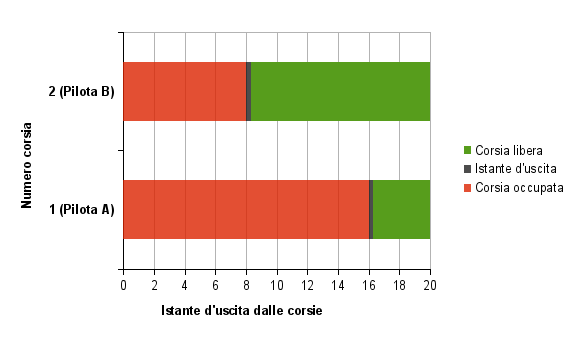
\includegraphics[width=110mm]{./Immagini/AccessoSegmentiStatoInziale.png}}
	% AccessoSegmentiStatoInziale.png: 575x338 pixel, 72dpi, 20.28x11.92 cm, bb=0 0 575 338
	\caption{Stato del segmento S all'istante in cui il pilota C chiede l'accesso}
	\label{fgr:AccessoSegmentiStatoInziale}
      \end{figure}
      
      Ora a seconda del valore di $T_i$ relativo al pilota A si possono ipotizzare tre possibili scenari, che sono
      
      \begin{itemize}
	\item $T_i < T_a$
	\item $T_a < T_i < T_b$
	\item $T_i > T_b$
      \end{itemize}
      
      Occorre anche introdurre un tempo chiamato $T_{min}$, ovvero il distacco minimo che 2 vetture possono avere
      stando sulla stessa corsia senza sovrapporsi. L'utilizzo di tale parametro verrà chiarito nella sezione
      \ref{Problemi legati alla granularita del tempo}
      
      Vediamo ora come si calcolerà il tempo d'uscita del pilota $P_c$ per ognuno di questi 3 casi.
      
      \subsection{Caso $T_i < T_a$}
	In questo caso il pilota $P_c$ uscirebbe sia prima di $P_a$ che di $P_b$, questo tuttavia non è possibile in quanto
	entrambe le corsie sono già occupate da piloti che la liberano dopo di lui in quanto $T_i < T_a < T_b$
	
	Il pilota $P_{c}$ verrà dunque inserito nella corsia con il tempo di uscita minore, ovvero $C_2$,
	e quindi attraverserà il segmento $S$ usando la corsia $C_2$ in tempo $T_r = T{c1} + T_{min}$
	uscendo subito dopo il pilota $P_2$. L'ordine d'uscita dal segmento sarà dunque $P_a -> P_c -> P_b$
	($P_c$ riesce a sorpassare $P_b$)
	
	Bisognerà poi aggiornare lo stato del segmento, ponendo l'aggiornamento dello stato del segmento ponendo
	$T_{C1} = T_{r}$ in quanto ora $P_c$ è l'ultimo pilota ad uscirà dalla corsia $C_2$, uno schema del
	nuovo stato del segmento è riportato nella figura \ref{fgr:AccessoSegmentiCaso1}
	
	\begin{figure}[h]
	  \centering
	  \fbox{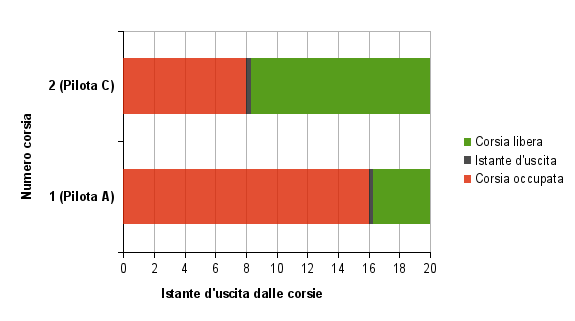
\includegraphics[width=110mm]{./Immagini/AccessoSegmentiCaso1.png}}
	  % AccessoSegmentiStatoInziale.png: 575x338 pixel, 72dpi, 20.28x11.92 cm, bb=0 0 575 338
	  \caption{Caso 1: Stato del segmento S dopo che il pilota C ha effettuato l'accesso}
	  \label{fgr:AccessoSegmentiCaso1}
	\end{figure}
	
      \subsection{Caso $T_a < T_i < T_b$}
	In questo caso il pilota $P_c$ uscirebbe dopo $P_a$ e prima di $P_b$, questo è compatibile con 
	lo stato del segmento in quando $P_c$ vede la corsia $C_1$ virtualmente libera poichè
	il pilota che la impegna esce in ogni caso prima di lui e non comporta nessun ostacolo alla sua percorrenza
	
	$P_c$ viene dunque inserito nella corsia con il tempo d'uscita minore, ovvero $C_2$ e dato che
	$T_i < T_{C2}$ potrà attraversare il segmento in un tempo $T_r = T_i$. 
	Nello stato della risorsa protetta del segmento verrà posto $TC_2 = T_r$, mentre $T_C1$ resterà invariato.
	L'ordine d'uscita dal segmento sarà poi $P_a -> P_c -> P_b$, e il pilota $P_c$ avrà effettivamente 
	superato $P_b$ come previsto.
	
	Uno schema del nuovo stato della risorsa protetta relativa al segmento $S$ è illustrato nella figura 
	\ref{fgr:AccessoSegmentiCaso2}

	\begin{figure}[h]
	  \centering
	  \fbox{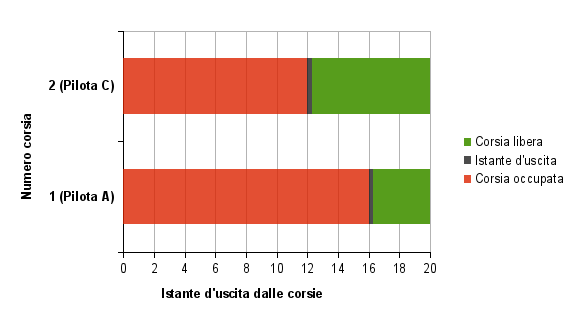
\includegraphics[width=110mm]{./Immagini/AccessoSegmentiCaso2.png}}
	  % AccessoSegmentiStatoInziale.png: 575x338 pixel, 72dpi, 20.28x11.92 cm, bb=0 0 575 338
	  \caption{Caso 2: Stato del segmento S dopo che il pilota C ha effettuato l'accesso}
	  \label{fgr:AccessoSegmentiCaso2}
	\end{figure}
      
      \subsection{Caso $T_i > T_b$}
	In questo caso il pilota $P_c$ uscirebbe sia dopo $P_a$ che dopo $P_c$, per lui il segmento
	è virtualmente libero in quanto nessuno dei 2 piloti gli crea intralcio. $P_c$ attraverserà
	dunque il segmento in tempo $T_r = T_i$ utilizzando comunque la corsia con il tempo d'uscita minore,
	ovvero $C_2$.
	
	Lo stato della risorsa protetta associata al segmento $S$ sarà modificata ponendo $T_C2 = T_r$,
	come rappresentato in figura \ref{fgr:AccessoSegmentiCaso3}, e l'ordine d'uscita sarà come previsto
	$P_a -> P_b -> P_c$.
      
	\begin{figure}[h]
	  \centering
	  \fbox{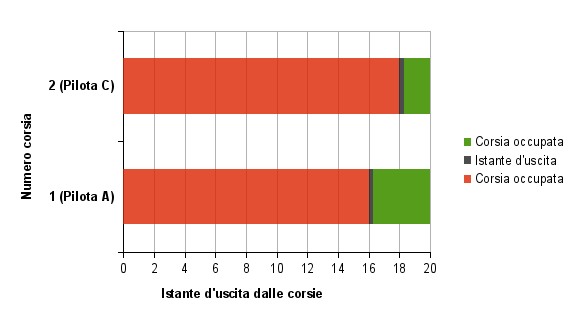
\includegraphics[width=110mm]{./Immagini/AccessoSegmentiCaso3.png}}
	  % AccessoSegmentiStatoInziale.png: 575x338 pixel, 72dpi, 20.28x11.92 cm, bb=0 0 575 338
	  \caption{Caso 3: Stato del segmento S dopo che il pilota C ha effettuato l'accesso}
	  \label{fgr:AccessoSegmentiCaso3}
	\end{figure}
	    
    \section{Stallo}
      Affinché in un sistema possa esserci possibilità di stallo devono verificarci queste 4 condizioni
      necessarie e sufficienti:
      
      \begin{enumerate}
       \item Accesso esclusivo a risorsa condivisa
       \item Inibizione di prerilascio
       \item Accumulo di risorse
       \item Condizione di attesa circolare
      \end{enumerate}
      
      Cerchiamo di analizzare ora queste 4 condizioni per determinare se nel sistema progettato
      possa esserci possibilità di stallo.
      
      \subsection{Accesso esclusivo a risorsa condivisa}
        Questa condizione è una parte fondamentale del sistema, in quanto non sarebbe possibile
	garantire uno stato coerente della competizione nel caso in cui 2 processi potessero accedere
	contemporaneamente allo stessa corsia dello stesso segmento modificandone lo stato.
	
	Riportandoci ad una caso reale sarebbe come se 2 vetture occupassero la stessa posizione nella stessa
	corsia di un segmento contemporaneamente,
	cosa ovviamente impossibile e da evitare.
	
      \subsection{Inibizione del prerilascio}
        Anche questa condizione non può essere evitata, in quanto sarebbe scorretto consentire ad un processo
	di potersi appropriare di una risorsa protetta in uso da un altro processo.
	
	Nel caso reale ciò sarebbe paragonabile alla situazione in cui un pilota eseguisse un sorpasso
	senza aver a disposizione una corsa libera. Anche questo deve essere vietato e quindi
	non è possibile rinunciare all'inibizione del prerilascio.
	
      \subsection{Attesa circolare}
        Data la natura circolare di un tracciato di Formula 1 esistono le condizioni necessarie affinché possa verificarsi 
	dell'attesa circolare, ma la dimensione del tracciato rapportata al numero di concorrenti fa si che questo 
	evento di difficile avvenimento.
	
      \subsection{Accumulo di risorse}
        Nel sistema progettato un processo per poter avanzare con l'esecuzione necessita
	al massimo dell'acquisizione di una sola risorsa protetta, quindi viene a mancare il caso in cui esso possa accumulare
	solo una parte di risorse attendendone altre prima di continuare.
      
      \subsection*{}
	In conclusione dato il non verificarsi della condizione di accumulo risorse possiamo affermare che il sistema
	progettato è esente da possibili stalli.    
    
    \section{Starvation}
      La starvation si verifica quando un processo non viene mai eseguito restando sempre in uno stato di wait.
      
      Nel nostro caso l'Utilizzo di politiche ad ordinamento temporale e gli accodamenti di tipo FIFO dovrebbero
      garantire un certa sicurezza al rischio di starvation.
      
      Inoltre i processi che rappresentano i vari piloti sono in stato di sleep per quasi tutta la loro esistenza,
      e non richiedono quindi un uso intensivo della CPU per poter eseguire garantendo la presenza di slot per
      eseguire altri processi.
    
    \section{Avvio e terminazione}
      Di seguito verrà spiegato come sono stati gestiti l'avvio e la terminazione dei vari componenti.
      
      Come già detto i 2 nodi devono poter eseguire in modo indipendente, anche se ovviamente
      è necessario che entrambi siano attivi per avere un completo funzionamento del sistema.
      
      \subsection{F1ControlPanel}
        Questo deve essere il primo nodo ad essere eseguito, in quanto pubblica lo IOR necessario al nodo F1Engine
	per poterlo contattare.
	
	\subsubsection{Avvio}
	  L'avvio del nodo non ha particolari aspetti rilevanti, in quanto si tratta semplicemente di un
	  pannello che visualizza le informazioni ricevute dall'altro nodo.
	  
	  Le operazioni eseguite sono:
	  
	  \begin{itemize}
	    \item Inizializzazione di Corba
	    \item Pubblicazione dello IOR
	    \item Creazione del pannello per visualizzare  dai ricevuti
	    \item Ascolto per la ricezione dei messaggi
	  \end{itemize}
	  
	\subsubsection{Terminazione}
	  Come per l'avvio anche la terminazione del nodo F1ControlPanel non ha aspetti molto rilevanti. 
	  La sua terminazione è infatti decisa dall'utente, in quanto siccome contiene tutte le informazioni
	  della gara è desiderabile che tali informazioni siano visibili anche al suo termine.
	  
	\subsubsection{Caduta o mancanza del nodo F1Engine}
	  Come detto la caduta del nodo F1Engine non ha ripercussioni sull'esecuzione di F1ControlPanel. Tale nodo
	  resterà comunque attivo anche se ovviamente non riceverà più alcun aggiornamento sullo stato della gara.
	  Potrà comunque essere utilizzato per visualizzare i dati di una nuova gara eventualmente avviata tramite un nuovo nodo
	  F1Engine.

      \subsection{F1Engine}
        Questo deve essere eseguito solo dopo aver avviato il nodo F1ControlPanel, in quanto necessita
	dello IOR da esso pubblicato per poter spedire i dati
	
	\subsubsection{Avvio}
	  L'avvio del nodo consiste nelle seguenti operazioni:
	  
	  \begin{enumerate}
	    \item Avvio del metodo main di F1Engine che invoca StartUp
	    \item Avvio del metodo StartUp che crea Gara e i task Piloti
	    \item Attesa dello schieramento dei piloti
	    \item Attesa del via da parte dell'utente
	    \item Partenza dei piloti
	  \end{enumerate}
	  
	  Nella figura \ref{Fig:Scope} sono chiariti gli scope dei vari componenti lanciati.
	  
	  \begin{figure}[ht]
	    \centering
	    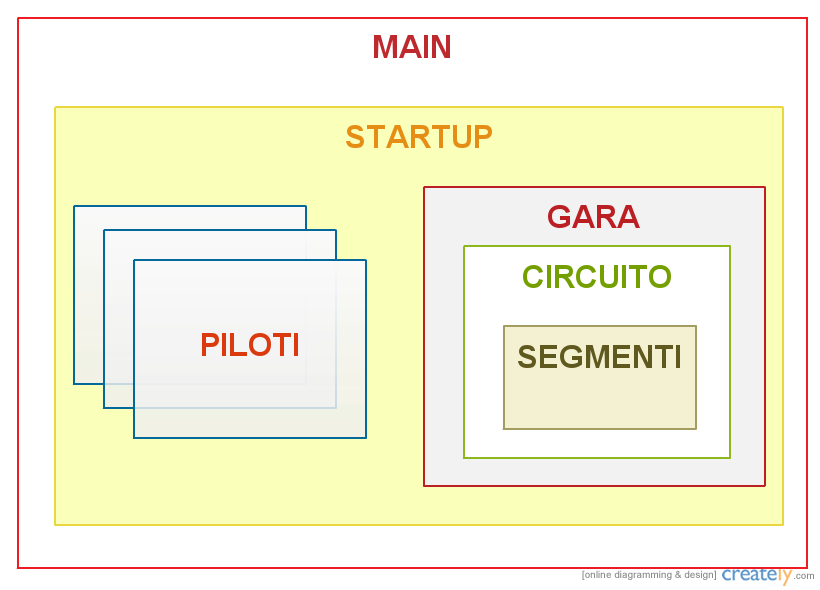
\includegraphics[width=120mm]{./Immagini/Scope.png}
	    % Scope.png: 820x590 pixel, 72dpi, 28.93x20.81 cm, bb=
	    \caption{Scope del nodo F1Engine}
	    \label{Fig:Scope}
	  \end{figure}
  
	\subsubsection{Terminazione}
	  La terminazione inizia quando tutti i piloti concludono la gara secondo questa serie di eventi:
	  
	  \begin{enumerate}
	    \item L'ultimo pilota conclude la gara e termina la propria esecuzione
	    \item A questo punto tutti i task creati da StartUp sono terminati
	    \item Gara non è più riferita da nessun componente al di fuori di StartUp
	    \item StartUp può terminare la sua esecuzione
	    \item Main ha invocato solamente StartUp, una volta che esso termina può a sua volta terminare
	  \end{enumerate}
	  
	  Il metodo main dunque termina dopo che tutti i piloti hanno concluso la loro gara, facendo così
	  terminare tutto il nodo F1Engine
	  
	\subsubsection{Caduta o mancanza del nodo F1ControlPanel}
	  La caduta o la mancanza del nodo F1ControlPanel non pregiudica il corretto svolgimento della gara,
	  semplicemente F1Engine continuerà la propria esecuzione senza però poter mandare alcuna informazione
	  sul proprio stato al monitor, ma visualizzando tali informazioni nel terminale anche se in modo 
	  poco pratico e non completo.
    
    \section{Problemi legati alla granularità del tempo}
    \label{Problemi legati alla granularita del tempo}
      Nelle prime esecuzione del sistema si sono notate delle problematiche relative alla granularità con cui
      il sistema operativo gestisce lo scorrere del tempo.
      
      Questo aspetto comportava il risveglio in ordine sbagliato dei piloti, dovuto al fatto che lo scheduler
      non riesce a gestire in modo corretto il risveglio di thread con istanti di risveglio molto vicini tra loro.
      Questo sostanzialmente comportava il verificarsi di sorpassi non possibili (ad esempio su segmenti con una sola
      corsia), e sono state pensate 2 possibili soluzioni per evitarli
      
      La prima soluzione consisteva nel creare un sistema di prenotazione in modo che un pilota potesse prenotare
      la mutua esclusione della risorsa protetta del segmento successivo. 
      Se la risorsa protetta associata ad un segmento riceveva la richiesta
      di mutua esclusione da parte di un pilota diverso dal primo in lista nell'elenco delle prenotazioni, allora tale pilota
      doveva essere riaccordato nella stessa coda. Tale processo di riaccodamento proseguiva finché il pilota
      che chiedesse l'accesso in mutua esclusione alla risorsa protetta fosse effettivamente quello in cima alla lista
      di prenotazione.
      
      Tale strategia, corretta dal punto di vista logico, comporta l'accumularsi di ritardi dovuti alla grande capacità
      di calcolo richiesta per eseguire un riaccodamento, in quanto si tratta di una operazione molto onerosa.
      
      La soluzione alternativa, che è quella che è stata poi implementata nel sistema, è molto più semplice
      ed è basata sul fatto che in una reale competizione i Formula 1 2 piloti su una stessa corsia
      non possono avere un distacco inferiore ad un certo limite, in quanto ciò significherebbe che essi sono sovrapposti.
      
      Anche nel sistema progettato è stato quindi inserito un distacco minimo tra i piloti, che garantisce 
      il fatto che 2 o più di essi non si risveglino mai in istanti così vicini da non essere ben gestiti 
      dallo scheduler.
      
      Varie prove hanno portato a scegliere come distacco minimo tra 2 piloti il tempo di 0.05 secondi.
	  
  \chapter{Implementazione}
    La presenza di 2 nodi distinti e con diverse funzioni ha portato a diverse considerazioni riguardo alla
    scelta dei linguaggi di programmazione da utilizzare nell'implementazione.
    
    \section {Nodo 1}
      Come già detto il nodo 1 contiene la gara, i piloti e il relativo StartUp e gestisce tutti gli aspetti
      legati alla concorrenza e alla temporizzazione.
      
      É stato quindi scelto di implementare questo nodo mediante il linguaggio ADA, che assicura un buon supporto sia
      riguardo alla concorrenza che riguardo alla distribuzione.
      
    \section{Nodo 2}
      Il nodo 2 ha caratteristiche del tutto diverse rispetto a quelle del nodo 1, in quanto non gestisce nessun aspetto
      legato alla concorrenza ma solamente quelli legati alla visualizzazione grafica.
      
      Per questi motivi è stato scelto di utilizzare Java per la sua implementazione, in quando garantisce un buon supporto
      all'aspetto grafico con la presenza di vari tool ne consente la progettazione mediante semplice drag-and-drop.
      Questo linguaggio garantisce inoltre un buon supporto alla distribuzione.
      
    \section{Middleware}
      Come Middleware è stato scelgo di utilizzare Corba, per via della sua diffusione e per il buon supporto dato
      ad entrambi i linguaggi usati
      
    \section{Accorgimenti}
      In fase di implementazione sono stati tuttavia necessari degli accorgimenti che hanno leggermente modificato la struttura 
      iniziale del progetto, riportato in figura \ref{Fig:SchemaDistribuzione}
      
      I problemi sono sorti quando più piloti utilizzano contemporaneamente il middleware Corba per 
      inviare messaggi al monitor, in quando
      ci sono state delle difficoltà nell'impostare Corba con una tasking policies che supportasse più thread per il lato ADA
      
      Per non superare ulteriormente il limite delle ore da dedicare al progetto si è scelto quindi di modificarne leggermente
      la struttura, introducendo una nuova entità chiamata Sender.
      
      Essa ha il compito si serializzare i messaggi inviati al monitor, in modo che non ce ne siano più di spediti
      contemporaneamente. Nella sua realizzazione è stata modellata come una risorsa protetta, con un procedura esposta per
      ogni tipo di evento che il pilota o lo StartUp può segnalare al monitor.
      
      %ovvero
      
      %\begin{itemize}
      % \item Add\_Pilot
      % \item Send\_Time
      % \item Enter\_Box
      % \item Exit\_Box
      % \item Send\_Circuiti\_Description
      % \item Send\_Start\_Race
      % \item Send\_Fuel\_And\_Tires
      % \item Send\_Finish\_Race
      %\end{itemize}
      
      Il fatto che si tratti di procedure garantisce che esse siano eseguite in mutua esclusione e quindi serializzate.
      Esse comunque devono solo consegnare il messaggio al middleware, usando ugualmente una politica best-efford
      e non introducono ritardi evidenti in fase di esecuzione.
      
      Lo stesso problema si è ripercosso anche nel nodo 2, in quanto poteva capitare che venissero chiamati
      più metodi del monitor allo stesso tempo causando degli errori nella visualizzazione.
      Anche questo è stato risolto eseguendo tutti i metodi per l'aggiornamento dell'interfaccia grafica in mutua esclusione,
      e anche in questo caso non ci sono ripercussioni in quanto nel peggiore dei casi l'unico inconveniente che si avrebbe sarebbe
      un leggero ritardo nell'aggiornamento dell'interfaccia grafica, difficilmente rilevabile e che non ne compromette
      la consistenza.
      
      Uno schema con l'architettura dopo l'introduzione dell'entità Sender è rappresentato nella 
      figura \ref{Fig:SchemaDistribuzioneSender}
      
      \begin{figure}[h]
	\centering
	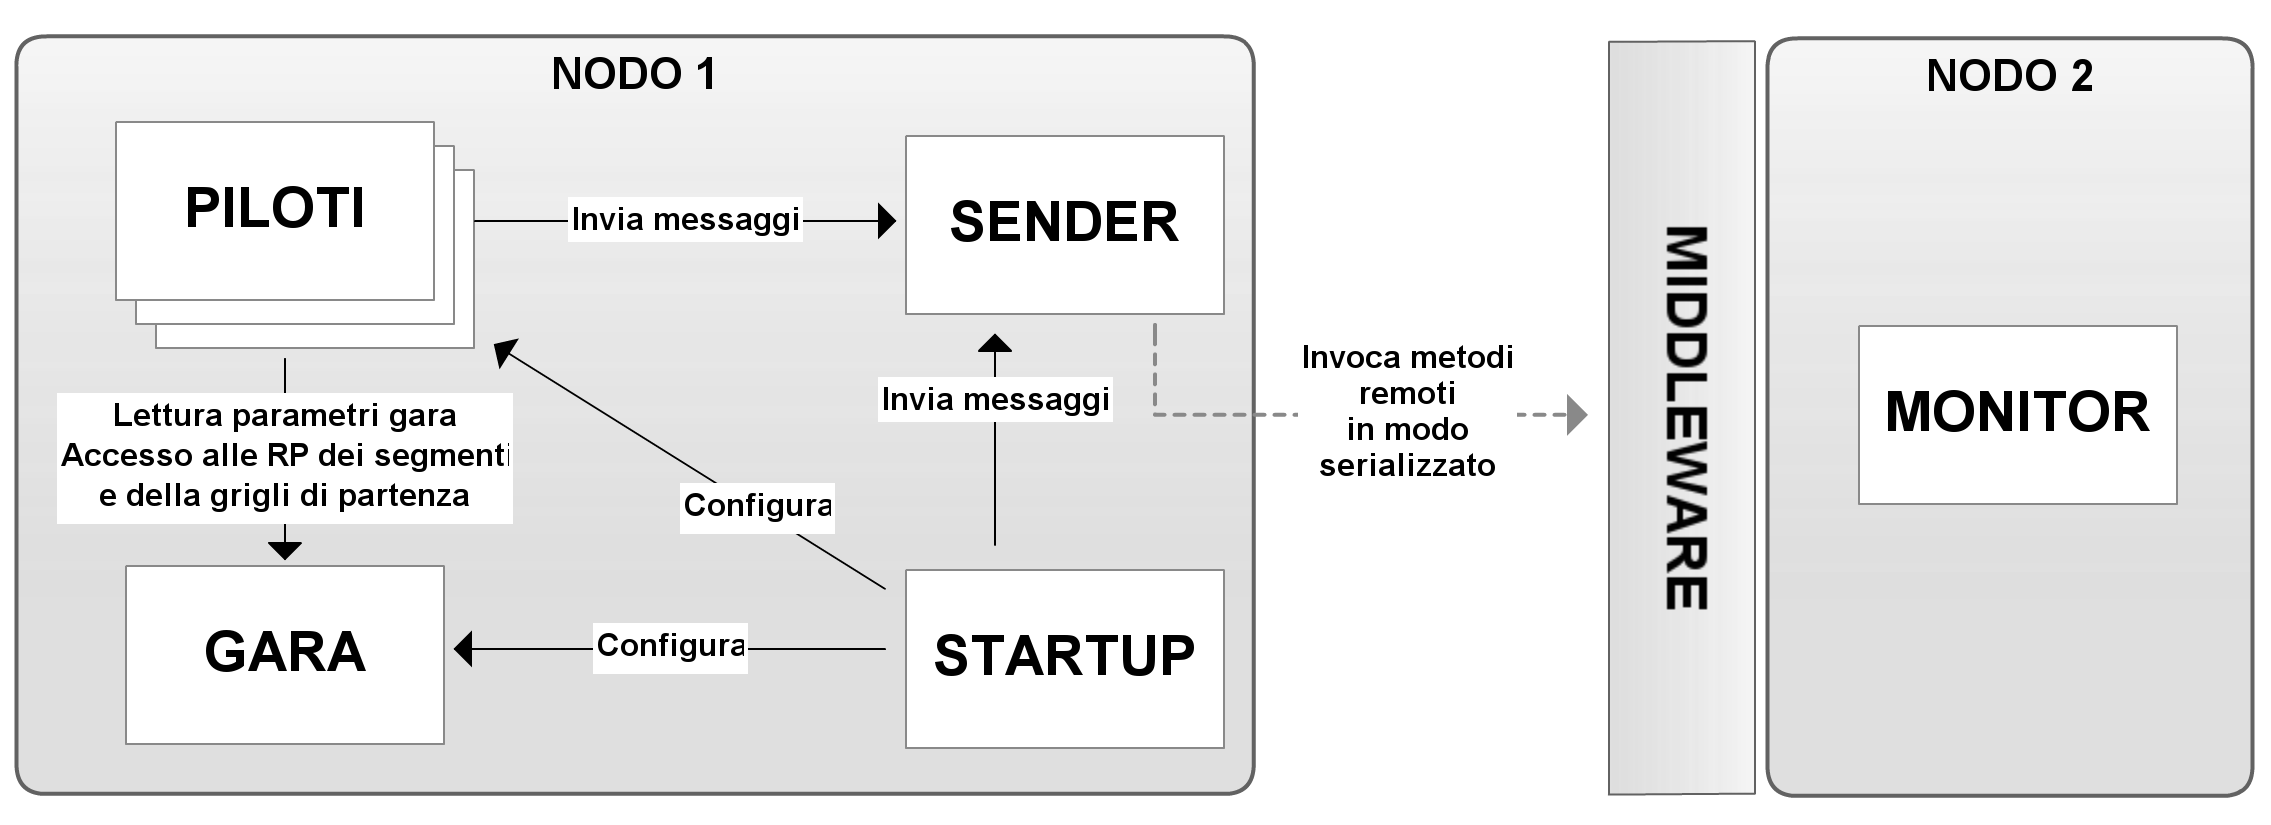
\includegraphics[width=120mm]{./Immagini/SchemaDistribuzioneSender.png}
	% SchemaDistribuzioneSender.png: 2178x792 pixel, 72dpi, 76.83x27.94 cm, bb=
	\caption{Schema di distribuzione dopo l'aggiunta dell'entità Sender}
	\label{Fig:SchemaDistribuzioneSender}
      \end{figure}      
      
  \chapter{Compilazione, configurazione ed esecuzione}
    \section{Ambiente d'esecuzione}
      Il progetto è stato testato sia su sistema operativo Ubuntu 13.04 che su sistema operativo virtualizzato Ubuntu 10.04.
      
      Oltre alle librerie standard del sistema operativo sono necessari i seguenti pacchetti:
      \begin{itemize}
        \item polyorb-server
	\item libpolyorb2
	\item oracle-jdk-7 o una distribuzione Java equivalente
      \end{itemize}

    \section{Compilazione}
      Nel progetto sono presenti 2 script, chiamati CompileEngine.sh e CompilePanel.sh
      che servono per compilare rispettivamente la partizione F1Engine e la partizione F1ControllPanel
      in modo indipendente.
      
    \section{Configurazione}
      Il progetto prevede tutta una serie di file di configurazione per personalizzare la competizione
      Questi file sono salvati nella cartella conf dell'F1Engine, e possono essere di 4 differenti tipi:
      
      \begin{itemize}
	\item file .trk, contenuti nella sotto cartella circuits\_set 
	\item file .car, contenuti nella sotto cartella cars\_set
	\item file .plt, contenuti nella sotto cartella pilots\_set
	\item file .conf, contenuti nella cartella conf
      \end{itemize}
      
      \section{File .trk}
	Ognuno di questi file descrive un circuito su cui è possibile svolgere una competizione, ogni riga contiene i parametri
	che descrivono un singolo segmento (quindi la prima riga contiene i parametri del primo segmento, la seconda
	quelli del secondo segmento e così via)
	
	I parametri per ogni segmento sono:
	\begin{itemize}
	  \item Segment\_Type (dec, acc, const, box)
	  \item Lenght (Integer 1..∞)
	  \item Speed (Float 1..∞) 
	  \item Num\_Lane (Integer 1..2)
	  \item Has\_Time\_Check (Positive 0..4)
	\end{itemize}
	
	\subsubsection{Segment\_Type}
	  Identifica il tipo di segmento (acc $=>$ accelerazione, const $=>$ curva, dec $=>$ decelerazione, box $=>$ box). 
	  I box devono occupare i primi 3 segmenti (decelerazione, box e accelerazione) e devono avere complessivamente una lunghezza
	  pari al segmento di partenza (che è alla terza posizione).

	\subsubsection{Lenght}
	  Indica la lunghezza del segmento in metri.

	\subsubsection{Speed}
	  Indica la velocità (m/s) massima in caso di un segmento di accelerazione, la velocità di uscita in caso di 
	  un segmento di decelerazione o la velocità di percorrenza in caso di segmento a velocità costante.
	  Se un segmento di accelerazione o di decelerazioneo precede un segmento a velocità costante, dovranno avere l'attributo 
	  Speed uguale.

	\subsubsection{Num\_Lane}
	  Indica il numero di corsie del segmento.

	\subsubsection{Has\_Time\_Check}
	  Indica se il segmento viene usato per la rilevazione dei tempi, devono essere in tutto 4. 
	  Indica anche il numero dell'intermedio.
      
      \section{File .car}
	Questi file di configurazione stabiliscono le possibili vetture che possono essere assegnate ai vari piloti.
	Ogni file definisce una vettura, e viene indicato un suo parametro per ogni riga col seguente ordine:
	
	\begin{itemize}
	  \item Manufacturer : String;
	  \item Coeff\_Acceleration : (Integer 1..10)
	  \item Coeff\_Deceleration : (Integer 1..10)
	  \item Max\_Speed: (Integer 1..100)
	  \item Coeff\_Roadholding: (Integer 1..10)
	  \item Coeff\_Tire\_Wear: (Integer 1..10)
	  \item Consuption: (Float 1..∞)
	  \item Max\_Fuel\_Level: (Float 1..∞)
	  \item Reliability: (Integer 1..10)
	\end{itemize}
	
	\subsubsection{Manufacter}
	  Indica la casa costruttrice della vettura.

	\subsubsection{Coeff\_Acceleration}
	  Indica il coefficiente di accelerazione, che è massimo se vale 10 e minimo se vale 1.

	\subsubsection{Coeff\_Deceleration}
	Indica il coefficiente di decelerazione, che è massimo se vale 10 e minimo se vale 1.

	\subsubsection{Max\_Speed}
	  Indica la velocità massima che l'auto può raggiungere in metri al secondo.

	\subsubsection{Coeff\_Roadholding}
	  Indica il coefficiente di tenuta, che è massimo se vale 10 e minimo se vale 1.

	\subsubsection{Coeff\_Tire\_Wear}
	  Indica il coefficiente di usura gomme, più alto è e meno si consumano.

	\subsubsection{Consuption} 
	  Indica il consumo dell'auto, misurato in litri per chilometro.

	\subsubsection{Max\_Fuel\_Level}
	  Indica la capienza del serbatoio in litri.
	  
	\subsubsection{Reliability}
	  Indica l'affidabilità della vettura.
      
      \section{File .plt}
	I file .plt descrivono un pool di piloti da cui è possibile scegliere quelli che effettivamente parteciperanno alla
	competizione.
	
	Ogni file descrive un diverso pilota, e in ogni riga si specifica una sua skill con il seguente ordine:
	
	\begin{itemize}
	  \item Name : (String);
	  \item Number : (Positive)
	  \item Skill\_Acceleration : (Integer 1..10)
	  \item Skill\_Deceleration: (Integer 1..10)
	\end{itemize}

	\subsubsection{Number}
	  Indica il numero del pilota.

	\subsubsection{Name}
	  Indica il nome del pilota.

	\subsubsection{Skill\_Acceleration}
	  Indica la skill di accelerazione, che è massimo se vale 10 e minimo se vale 1.

	\subsubsection{Skill\_Deceleration}
	  Indica la skill di decelerazione, che è massimo se vale 10 e minimo se vale 1.
	  
      \section{File .conf}
	Ognuno di questo file descrive una competizione. Nella prima parte si specificano, uno per riga,
	le seguenti opzioni della competizione:
	
	\begin{itemize}
	  \item Nome del file con la configurazione del circuito
	  \item Numero di giri previsti (Positive)
	  \item Condizioni meteo (dry, wet)
	\end{itemize}
	
	Nella seconda parte del file invece si elencano tutti i piloti che partecipano alla competizione, 
	specificando quale vettura è a loro assegnata, la quantità di benzina a inizio gara e i giri in cui 
	entrare a i box per cambiare gli pneumatici.
	
	Per ogni riga verranno dunque indicati:
	\begin{itemize}
	  \item Nome del file del pilota
	  \item Nome del file della vettura assegnata al pilota
	  \item Litri di benzina caricati a inizio gara (Positive)
	  \item Elenco dei giri in cui fermarsi ai box (Elenco di Positive)
	\end{itemize}

        Nel progetto sono già inclusi vari file di configurazione, con la quale è possibile testare il tutto.
        Il file test\_1lane.conf contiene una configurazione che avvia una competizione senza soste ai box
	in cui il circuito è interamente ad una corsia,
	e nonostante la presenza di auto lente nelle prime posizioni si può notare come esse facciano da tappo
	in quanto su tale tracciato non è possibile eseguire sorpassi.
	
	Il file test\_2lane.conf avvia invece una competizione con soste ai box in un circuito con la presenza alcuni di segmenti
	con 2 corsie, dove si può notare l'esecuzione di sorpassi ai danni dei piloti più lenti.
	
    \section{Esecuzione}
      Per semplificare la fase di test si ipotizza che entrambi i nodi siano eseguiti sullo stesso terminale, in modo che lo IOR 
      del server dei nomi possa essere condiviso mediante un semplice file di testo accessibile da entrambi i nodi.
      
      Nel progetto sono presenti 2 script per lanciare il software. 
      
      Per prima cosa bisognerà avviare lo script con nome StartControlPanel.sh che ha il compito di avviare il pannello
      per la visualizzazione delle statistiche e il server dei nomi per il la distribuzione.
      
      Una volta avviato il pannello sarà necessario lanciare lo script StartEngine.sh, che si occuperà di avviare il nodo F1Engine
      usando lo IOR precedentemente salvato dal nodo F1ControlPanel.
      Lo script StartEngine.sh deve inoltre ricevere in ingresso una stringa contenete il nome del file .conf
      desiderato.
      
      Un esempio di una possibile esecuzione partendo dalla cartella Workspace del progetto è la seguente:
      
      \begin{xml}
        cd F1ControlPanel
	sh StartControlPanel.sh
	cd ..
	cd F1Engine
	sh StartEngine.sh test_2lane.conf
      \end{xml}

\end{document}
